\documentclass[12pt]{article}
\bibliographystyle{unsrt}
\usepackage{a4}
\usepackage{graphicx}
\usepackage{url}
\usepackage{color}
\newcommand{\ca}{\mbox{C$\alpha$}}
\newcommand{\VH}{\mbox{V\kern-.1667em \lower.5ex\hbox{\scriptsize H}}}
\newcommand{\VL}{\mbox{V\kern-.1667em \lower.5ex\hbox{\scriptsize L}}}
\newcommand{\VHVL}{\mbox{\VH/\VL}}
\newcommand{\CH}[1]{\mbox{C\lower.5ex\hbox{\scriptsize H}#1}}
\newcommand{\CL}{\mbox{C\kern-.0833em \lower.5ex\hbox{\scriptsize L}}}
\newcommand{\FV}{\mbox{\it Fv}}
\newcommand{\Fab}{\mbox{\it Fab}}

\newcommand{\e}[1]{\mbox{$\times 10^{#1}$}}
\newcommand{\etal}{~\emph{et al.}}
\newcommand{\degree}{\mbox{${}^{\circ}$}}
\newcommand{\lilian}[1]{ {\color{red}{\bfseries Lilian:} #1}}
\newcommand{\andrew}[1]{ {\color{green}{\bfseries Andrew:} #1}}
\newcommand{\rewrite}[1]{{\color{blue}{\bfseries Andrew to rewrite:} #1}}

\usepackage{soul}
\newcommand{\highlight}[1]{\hl{#1}}
% \newcommand{\highlight}[1]{{\color{cyan} #1}} % Use this if soul package not available!

\let\shortcite\cite
\emergencystretch 1in

\title{Predicting the Quality of CDRH3 Antibody Loop Structural Models}
\author{Lilian M.\ Denzler and Andrew C.R.\ Martin\\
Structural and Molecular Biology, Division of Biosciences,\\
University College of London,\\
Gower Street,\\
London WC1E 6BT, UK
}

\begin{document}
\maketitle

\begin{abstract}
  Therapeutic antibodies have shown an unprecedented pace of
  development and have brought new hope for the treatment of numerous
  diseases. Bioinformatics tools for modelling antibody structures
  have become invaluable for antibody engineering and the development
  of therapeutic antibodies. The antigen-binding site consists of six
  hypervariable loops, also known as the Complementary Determining
  Regions (CDRs), all of which can be modelled with adequate accuracy,
  except for one. It remains remarkably difficult to model the third CDR
  loop of the antibody heavy chain. CDR-H3 has
  far greater length and sequence variability, with such great structural
  diversity, that modelling it is considerably harder.

  Many approaches for antibody modelling, such as our
  abYmod software, have been developed. Although such efforts have
  improved prediction accuracy the results for CDR-H3 are
  still inconsistent and require further improvement. Providing a
  confidence score for the structure predictions would aid in
  differentiating well-modelled structures from incorrectly modelled
  structures, giving the abYmod user a clearer understanding of the
  generated 3D-model reliability.

  We present a 3D-model quality predictor, combining domain knowledge
  with machine learning techniques to predict the accuracy of CDR-H3
  3D-models generated by antibody modelling software such as abYmod. The
  newly developed predictor scored a Matthews Correlation Coefficient
  of 0.99, and can thus be described as highly reliable. The predictor
  is made available at \url{http://www.bioinf.org.uk/abs/qualiloop/}
\end{abstract}

\section{Introduction}

Antibodies are highly specialized proteins of the immune system that
are produced in response to a foreign substance, called an antigen. A
mature antibody binds a specific antigen with high affinity, while
only weakly interacting with other antigens, or not at all. This high affinity and high specificity sets them apart from other pharmaceuticals and makes them effective drugs with endless possibilities in application given their ability to target an immense variety of antigens.
Furthermore, in contrast with small drug molecules, antibodies can not
only bind pockets, but also flat, concave or convex
surfaces\cite{MacCallum1996}. Their unique characteristics have enabled 
researchers to develop efficient antibody drugs for treating cancers,
autoimmune disorders, infectious diseases and many more\cite{Lu2020}.
Four of the top 10 best-selling drugs in
2020 were monoclonal antibodies\cite{Urquhart2021}.

In order to design therapeutic antibodies rationally, knowledge of
their structure is essential. The acquired structural information can
be used to increase binding affinity to a target of interest,
predicting both the exact binding site and the antibody stability as
well as assessing immunogenicity\cite{Abhinandan2007}. As
experimental structure determination is costly and time
consuming, computational predictions of an antibody's structure are
used to streamline the process.

The variable
fragment (Fv) of an antibody contains the six complementarity determining regions
(CDRs, also known as hypervariable loops) which form the antigen binding site.
All except one of these loops can be clustered
into a limited number of `canonical structures'\cite{Al-Lazikani}. Therefore, modelling
these loops with adequate accuracy is commonly
achievable\cite{North2011}.  However, the CDR loop 3 of the 
heavy chain (CDR-H3) has a far greater sequence variability due to the
processes of V(D)J recombination and somatic hyper‐mutation and its
structure has remained unclassifiable\cite{Finn2016}. The variety in
structure is so great, that its structural diversity is remarkable
even compared to other protein loops\cite{Regep2017}. It was found
that over 75\% of CDR-H3 loops do not have a sub-{\AA}ngstr\"{o}m non-antibody
structural neighbour, while 30\% of CDR-H3 loops have a
completely unique structure compared with under 3\% for all non-antibody
loops\cite{Regep2017}.

Apart from being the most structurally diverse, the CDR-H3 loop is
also the most important for antigen binding, being located at the
centre of the binding site and forming the most contacts with the
antigen\cite{MacCallum1996}. It was demonstrated that
differences in this loop alone are sufficient to enable otherwise
identical antibodies to distinguish between various
antigens\cite{Xu2000}.

According to the Kabat definition, the CDR-H3 loop is made up of the
residues 95--105 (using the Kabat\cite{Kabat1992}, Chothia\cite{Al-Lazikani} or Martin\cite{Abhinandan2008} numbering schemes) in the heavy
chain, with a potential insertion site at position 100. The
possibility of such an insertion of a varying number of residues leads
to a large range of loop lengths, with bovine antibodies being
exceptionally long (Figure~\ref{fig:loopdist}).

For shorter loops, a higher prediction accuracy can be achieved than
for longer CDR-H3 loops. This was also shown by the Antibody Modelling
Assessments (AMA), two blind contests that required researchers to
build three-dimensional structural models (3D-models) from antibody sequences. The CDR-H3 loop
modelling quality achieved at the contests was on average much lower
for loops of longer lengths\cite{Almagro2011,Almagro2014}.

Several different approaches for generating 
3D-models from antibody sequences exist such as
RosettaAntibody\cite{Sircar2009,Sivasubramanian2009}, 
ABodyBuilder\cite{Leem2016}, PIGSPro\cite{Lepore2017}, Lyra\cite{Klausen2015}, AbLooper\cite{Abanades2022} and our own abYmod.
One of the most
used methods is RosettaAntibody, which implements template selection
and \emph{ab initio} CDR-H3 loop modelling using loop fragments and employing
specific angle restraints which bias the conformational space towards
so-called `kinked' loops\cite{Schoeder2021,Weitzner2017}. In
contrast, ABodyBuilder uses a database search algorithm
(FREAD\cite{Choi2010}) for CDR loop modelling.
abYmod \url{http://abymod.abysis.org/} utilizes extensive canonical
class definitions, \VHVL\ angle prediction and a large database of loop
structures (LoopDB) for CDR-H3 modelling.
Upon inputting an antibody sequence, abYmod assigns the
canonical class using a set of key residues\cite{Martin1996} and where
an exact match is not possible, a nearest class is identified.

abYmod selects light and heavy chains separately from PDB templates.
First these are selected on the basis of the number of matched
canonical classes and then on the basis of sequence identity.  The
\VHVL\ packing angle is currently selected from the parent that has
the best sequence identity over both chains, but an improved method is
currently in development. Any CDRs where there was no canonical match are then
are grafted onto the framework. If there is no template of the correct
length for CDR-H3, the loop is built using LoopDB, a database of
CDR-H3-like loops from all proteins. Finally, Gromacs energy
minimization software is used to optimize the 3D-model. This method has
proven very effective and preliminary analysis suggests the method
achieves comparable results, or outperforms, other modelling software
(see Results).

Using these mentioned modelling methods, framework regions can
generally be predicted with great accuracy (with better than 1\AA\
RMSD\cite{Almagro2014}), as one can often find a very similar
structure for the homology modelling process.  However, the CDR loops
are not as easily predicted due to their great diversity. If the
canonical conformation of CDR loops CDR-L1,L2,L3,H1,H2 can be identified, they too
can be modelled rather well, often within 1\AA\ \ca~RMSD, for CDR-H3 loops
the The average values are taken from the antibody modelling assessment average is usually above 3\AA\cite{Almagro2011}.

ABodyBuilder is a modelling server that provides the user with a
confidence score for each region (e.g.\ CDR-H2) of the antibody
3D-model. The given score is the probability that a specific region
(e.g.\ CDR-H2) will be will be modelled within a specific RMSD
threshold\cite{Leem2016}. Thus, it can be used to obtain an expected
RMSD value for a given probability (default 75\%). For the CDR-H3 this
score is calculated as a function of the loop length.  The confidence
scorer is described as robust, but less accurate in the case of CDR
loops due to the lack of data\cite{Leem2016}. ABLooper also provides a
confidence metric for the CDR-H3 loop 3D-model, which is estimated by the
diversity of a set of predicted conformations for the same
loop\cite{Abanades2022}. However, it remains unclear whether a high
prediction diversity score points towards loops with multiple
conformations or a low quality 3D-model. Furthermore, it remains unclear
how well the generated diversity score reflects 3D-model
quality\cite{Abanades2022}.


Modelling the CDR-H3 loop is a hurdle for \emph{in silico} development of
therapeutic antibodies. Currently, there is no definite, reliable way
to determine how accurate a generated structural 3D-model is within the
H3 region. Therefore, we have produced a
user-friendly predictor of CDR-H3 3D-model quality. The predictor will give
the user an RMSD-range in {\AA}ngstr\"{o}ms, in which the generated 3D-model lies
with a high probability.
This information can guide the
user in the antibody engineering process. The user has the choice to
determine whether the 3D-model is to be used as is, or
whether the 3D-model should be re-worked.

\section{Results}

The predictive power of any machine learning model (ML-model) is largely
dependent on the quality and size of the dataset on which it was trained. As
this is a non-linear, complex, multi-class classification problem, a
substantial amount of data was required. Thus, an extensive, verified
dataset of antibody structures called abYbank/AbDb\cite{Ferdous2018},
was utilised (1924 non-redundant
structures). The \ca\ root-mean-square deviation (RMSD) value
between the crystal structures
and modelled structures was calculated (see Methods) and
was used to classify 3D-models.

\begin{figure}
  \centering
  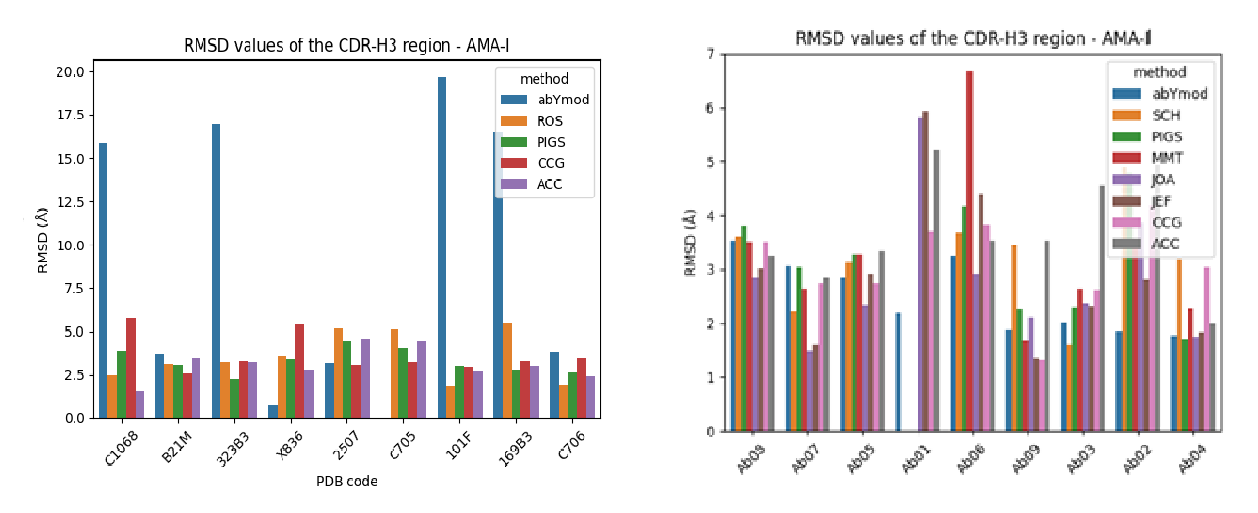
\includegraphics[width=\linewidth]{AMA.eps}
  \caption {RMSD values of the CDR-H3 loop for structures from the
    Antibody Modelling Assessment I (2011) and AMAII (2014). abYmod
    outperforms other modelling software in some instances, but also
    has much lower accuracy in few outlier cases. Left: an abYmod
    structure for C705 could be generated, yet the RMSD calculation
    failed \lilian{Why? I'm sure we can resolve this!}.
    Right: Ab01 is the rabbit antibody PDB:4MA3, which was
    excluded in the CDR-H3 modelling stage in AMAII due to
    difficulties modelling the overall structure previously. Ab01 is
    shown for the methods, where generated 3D-models were adequate for
    RMSD calculation. \lilian{This needs better explanation}}
  \label{fig:AMA}
\end{figure}

The full pipeline for creating the final ML-model
starts with 
feature-set calculation using the antibody sequence. The feature set
includes attributes linked to sequence, structure, physical
characteristics, interactions, etc., within, as well as outside, the
loop. 
The sequence logo (Figure~\ref{fig:logo}) visualizes amino acid
occurrence within the loop sequence, elements of which can be
extracted as features \cite{Thomsen2012,Shaner1993}.

\begin{figure}
  \centering
  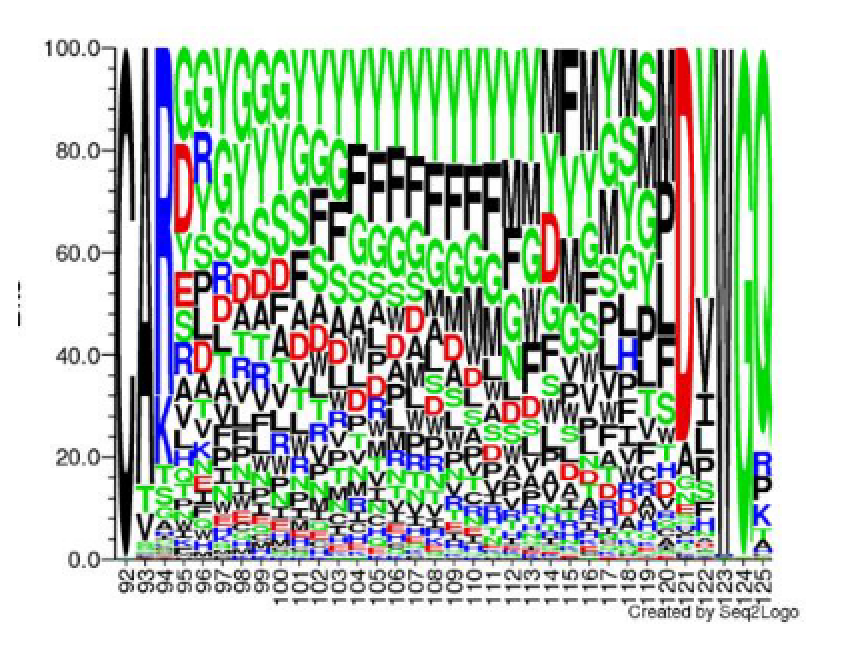
\includegraphics[width=\linewidth]{logo.eps}
  \caption {Sequence Logo of the CDR-H3 loop sequence. Data on amino
    acid occurrence taken from \protect\url{http://abymod.abysis.org/} Visualized
    using Seq2Logo using Kabat Numbering}
  \label{fig:logo}
\end{figure}

After creating the feature dataset, it is pre-processed (cleaning,
scaling, encoding, see methods for details). Structures with a
resolution worse than 4\AA\ were removed.
Instances of antibodies in our non-redundant dataset that matched in loop sequence were
not removed. 3D-Models of some of these structures with the same loop
sequence differ significantly. The few large RMSD ranges may stem from
low resolution. For example, the loop sequence with the largest RMSD range 
has multiple structure files linked to it of varying quality, one of which has a resolution of only 3.00\AA. Residue differences near the loop may also
explain the conformational difference of the loop itself, 
even if the loop sequence does not differ. Some of these structures are
complexed while others are not, which may also affect the loop
structure (manuscript in preparation).


The target data (i.e.\ RMSD values) are transformed from numerical
values to nominal values so that they can be used for
classification. In order to define these nominal categories, the total
RMSD range must be divided into categories. This is done either by
creating uniform classes i.e.\ 1--2\AA, 2--3\AA, etc., (the optimal size of which
must be determined), or by creating balanced classes. When
creating balanced classes, the upper and lower thresholds of a
category are chosen in such a way that each class contains an equal
number of instances. This approach was chosen to counteract the
skewness of the RMSD distribution. However, this was found to
affect the final ML-model's predictive power negatively. Therefore,
uniform classes were used.

The RMSD values are also transformed into a set of binary values according to a
list of RMSD thresholds (i.e. a 1 is assigned to above and 0 to below a given threshold). This is done so that binary ML-models can be
trained, which will predict the probability e.g.\ that the 3D-model's RMSD
is above 2\AA, 2.2\AA, 2.4\AA, and so on. The number of binary
classifiers incorporated into the first layer has a great effect on
the final ML-model, the general trend being that the more binary
classifiers are used, the better the nominal prediction. \lilian{Data?}

\subsection{Feature Encoding and Selection}

As some features are in the form of amino acid names, these must be
encoded before they can be passed to a ML-model. The
encoding strategy often determines how efficiently the ML-model learns
and how much information can be extracted. Different strategies were
employed to represent protein sequences numerically, such as BLOSUM62\cite{Henikoff1992} and NLF\cite{Nanni2011} encoding (a non-linear Fisher transform of a large set of physicochemical properties). The four-feature physiochemical encoding strategy\cite{Abhinandan2010} was implemented for all ML-models, being
the most effective. However, PCA-3 BLOSUM62, a dimensionality-reduced
BLOSUM62 encoding method achieved comparable results.
Feature selection was conducted to improve the ML-model's learning
capacity. A high-dimensional feature dataset bears the risk of
introducing excessive noise, facilitating ML-model over-fitting and can be
responsible for an overall decrease in ML-model performance and
stability. Each additional input feature forces the ML-model to
handle a more complex task, which consumes excess computational power
and time and provides more variables leading to over-fitting of the ML-model.

Our ML-model was trained on different feature sets selected using manual
selection as well as algorithmic selection strategies (see methods), in order to
determine the most effective feature selection method. None of the
feature selection methods was a best fit for all ML-models. To create a ML-model implementing the encoding and feature selection strategies best suited for the specific ML-structure, a number of different combinations were tested, summarized in \ref{fig:results_table}.
\begin{table}[results_table]
    \centering
    \begin{tabular}{c|c}
         &  \\
         & 
    \end{tabular}
    \caption{Summary of Results of different ML-model implementations.}
    \label{tab:my_label}
\end{table}

\lilian{So, having read this, I have no idea what feature encoding you
  actually used, or where to find that information. What worked and
  what didn't? Where can I find a comparison of the performance?}

After the data were processed, they were used to train different
ML-models. Different types of ML-model were investigated, as the most
suited ML-model type has to be determined heuristically. 
The following list, which includes some of the most commonly used
algorithms, was used: logistic regression, linear discriminant analysis,
K-nearest neighbours classifier, decision tree classifier, Gaussian
NB, random forest classifier, support vector machine,
probability-based voting (also known as soft voting) and extreme
gradient boosting (XGBoost)\cite{Chen2016}.
\lilian{OK, but this is the Results section, so where are the results
  of using the different methods?}

The best ML-model, and its best hyperparameters, are then determined for
each binary RMSD target. The set of binary ML-models outputs a number of
predictions that give the likelihood of the 3D-model having an RMSD above
the threshold value of the respective ML-model. These predictions are
then added to the feature set, on which a top-layer classifier is then
trained (Figure~\ref{fig:method}). Thus, a quasi-voting-system is incorporated into the final
classifier, in which a set of weaker classifiers vote on the ML-model
quality.

\subsection{Hyperparameter Optimization}
In the process of hyperparameter optimization, the configuration of
ML-model parameters which results in best performance is selected. This
is usually a computationally expensive and manual procedure.
In an effort to automate this process, a population was defined for
each ML-model type, so hyperparameter optimization could be conducted
automatically for each ML-model and seamlessly integrated into the full
ML-model creation process. Two different methods for hyperparameter
optimization were tested. The first was a hybrid approach of randomized
search and grid search; the second used a genetic algorithm for
optimization. The genetic algorithm was found to achieve slightly
better results and was employed for optimizing all ML-models.

\subsection{Machine Learning Model Performance}
The overall best final ML-model was composed of several different binary
classifiers,\lilian{More detail!} with an extreme gradient boosting (XGBoost) top-layer
nominal classifier. Features were selected using random forest feature
selection.
\lilian{Explain how this works and which features were selected --- and how many?}
A final MCC\lilian{Explain how MCC is calculated over 3 classes} value of 0.99 could be achieved for an ML-model
using the abYmod log file \lilian{What parameters are actually used?} as input as well as the loop 3D-model file
itself. This value slightly dropped to 0.92 if no such log file was
given. This is mainly\lilian{is there anything else?} due to the fact that the template sequence
abYmod used to generate the 3D-model is unknown in the latter case.

\lilian{I'm not sure this is in the most logical place --- isn't this
  something that was chosen at the start? (At least in terms of
  telling the story}
The classifier predicts whether a 3D-model has an RMSD of below 2\AA,
between 2--4\AA, or above 4\AA. These cutoff values were selected
based on the observation that abYmod generally produces a 3D-model with
RMSD below 4\AA. Incorrectly modelled structures (Figure~\ref{fig:AMA}) may
be identified by screening for structures estimated to have an RMSD
above 4\AA. If a very high-quality 3D-model is needed one should also
exclude 3D-models with RMSD above 2\AA.

The software
was tested on a test-set of antibody structures used in the 2014 and
2011 Antibody Modelling Assessments
\cite{Almagro2011,Almagro2014}. As the results depicted in
Figure~\ref{fig:AMA} show, abYmod achieves results similar to, or better than,
other modelling programs. However, the outliers with very high RMSD
values increase abYmod's RMSD average. The predictor in this work
would aim to identify such outlier 3D-models.


\section{Methods}

\subsection{Computing}
All machine learning, feature selection and hyperparameter
optimization algorithms were implemented in Python. The Scikit-learn
library was used for training ML-models, the
Yellowbrick\cite{Bengfort2021} library was utilized for
visualization. All code is available at
\url{https://github.com/LilianDenzler/qualiloop}

The code was run under CentOS 7 on an 8-core virtual machine on an
Intel Xeon 4208 CPU with 16Gig RAM.

\subsection{Data Pre-Processing and Preparation}
Handling Null Values and Duplicates: The dataset containing target
RMSD values, and the calculated features was screened for null
values.
Rows that contained any null values were
removed from the dataset (11 rows in total).

\subsubsection{Duplicate Screening}
Using AbDb's redundancy information it was ensured that no antibodies
were present in the dataset more than once. \highlight{The dataset was
  additionally screened for duplicate instances.}
\lilian{Did you find any? How was this screening done? It's far from trivial}

\subsubsection{Scaling}
Normalization and Standardization\lilian{What's the difference? Explain what they are.} were tested as scaling methods. Both
approaches are greatly influenced by outliers, and such datapoints are
ideally removed for optimal scaling. Here we define outliers as
datapoints that lie over 1.5 times the interquartile range (IQR) below
the first quartile or above the third quartile. The IQR is defined as
the range between quartile 1, i.e.\ the median of the lower half of the
data, and quartile 3, i.e.\ the median of the upper half of the
data. However, across all features there are a total of 632 outlier
values and removing such a large number of datapoints is not a viable
option. A robust scaler\cite{XXXX} was also used, which uses statistics that are
robust to outliers. The median is set to zero and numerical features
are scaled to the interquartile range.

\subsubsection{BLOSUM 62 Encoding}
The BLOSUM62 matrix reflects the frequencies of amino acid
substitutions within a locally aligned, conserved regions of proteins
with at least 62\% similarity. Each amino acid is represented by a row
(or column) of the BLOSUM62 matrix. Dimensionality reduction
techniques were employed: Principal Component Analysis (PCA),
Independent Component Analysis (ICA), projection-based methods (t-SNE,
Isomap). Three components were used as features. PCA was found to be the most effective dimensionality reduction method. 

\subsubsection{Physiochemical Feature Encoding}
Martin and Abhinandan\shortcite{Abhinandan2010} introduced an encoding using
four physiochemical features:
the total number of sidechain atoms; the
number of sidechain atoms in the shortest path from the \ca\ to the most
distal atom; the Eisenberg consensus
hydrophobicity\cite{Eisenberg1982}; the charge (using +0.5 for histidine).

NLF-encoding \shortcite{Nanni2011} describes a new peptide encoding technique optimized for use with machine learning classifiers. A non-linear Fisher transform is applied to the whole set of physiochemical properties in \shortcite{Kawashima2000}
physiochemical properties are calculated and transformed using a
non-linear Fisher transform for dimensionality reduction.  A vector of
length 19 is produced for each amino acid.



\subsubsection{NLF Encoding}
This method of encoding is detailed by Nanni and Lumini in their paper. It takes many physicochemical properties and transforms them using a Fisher Transform (similar to a PCA) creating a smaller set of features that can describe the amino acid just as well. There are 19 transformed features. 

\subsection{Dataset-splitting}
The final ML-model was evaluated using a test set, separated from the
training set at the start in a 30/70 split. The performance of all individual sub-ML-models of the first layer was determined using stratified K-folds cross-validation (K=10) as the
dataset is imbalanced, being skewed towards lower RMSD values\cite{Krstajic2014,Kohavi1995}. The
method is different from normal K-folds cross validation as it uses
stratified sampling, which is also random, but selections are made to represent class imbalance.
This ensures each class is represented, as the percentage of samples for each class is
preserved.

\subsection{Machine Learning Model Assessment} 
ML-Model assessment must be considered at two levels as performance
metrics of binary and multi-class classifiers are calculated
differently and must thus be considered separately. The Matthews
Correlation Coefficient (MCC)\cite{Chicco2020} is deemed the most
informative, taking the ratios of the four confusion matrix categories
into account and is thus more reliable than the F1 score and
accuracy. It is also consistent for both binary and multi-class
problems and therefore well suited for our purpose.\cite{Jurman2012}
 
\subsection{Feature Calculations}
\begin{figure}
  \centering
  \includegraphics[width=\linewidth]{feature_table.eps}
  \caption {A summary of how different feature values were calculated. \lilian{It's a table! Why import it?}}
  \label{fig:feature_table}
\end{figure}

\begin{figure}
  \centering
  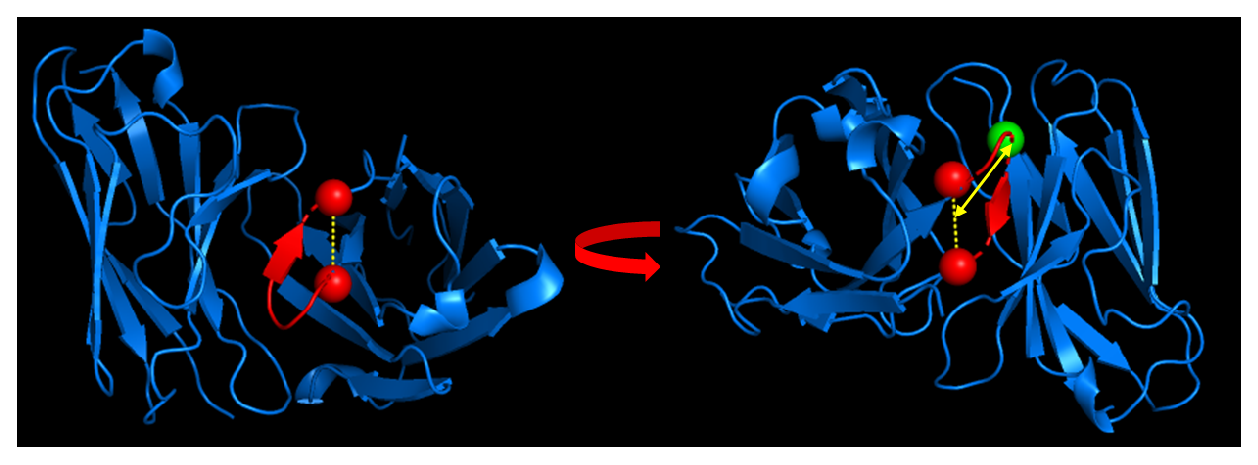
\includegraphics[width=\linewidth]{angle.eps}
  \caption {Diagram \lilian{Needs a much simpler cartoon diagram --- it's difficult to see anything from this!}
    visualizing the process underlying the protrusion
    calculation. First, the base residues (i.e.\ H95 and H102, shown as
    red spheres) of the CDR-H3 (shown in red) are identified. Then, a
    line is drawn between the two \ca\ atoms of these residues (yellow
    dashed line). The distance of the \ca-atom of each residue in the
    CDR-H3 loop to this line is calculated. The residue which has the
    greatest distance to the line (shown as green sphere) is output
    as one-letter amino acid code and used as feature. The distance in
    \AA\ (depicted as yellow arrow) is used as the `protrusion'
    feature. \lilian{It's unclear whether you use both distance and amino acid, or just one of these.}}
  \label{fig:angle}
\end{figure}




\section{Discussion}
The results suggest that our classifier can differentiate
between well-modelled and less well-modelled CDR-H3 loop
structures. An MCC value of 0.99 was achieved, which underlines this
ability for accurate discrimination. Different methods for data
pre-processing, feature encoding, feature selection and hyperparameter
optimization were tested.
Feature encoding methods that were very high-dimensional
(one-hot-encoding, BLOSUM62, NLF) were found to be
unfavourable. Dimensionality reduction methods (Principal Component
Analysis (PCA), Independent Component Analysis (ICA), projection-based
methods e.g.\ t-SNE) were used on BLOSUM62 encoded matrices, which lead
to significant improvement. However, a physicochemical encoding
strategy was most effective.
The selection of features incorporated in the training set seemed to
be most important for effective learning. A multitude of methods were
tested. No one fit-for-all method for the different ML-models could be
found.\lilian{I'm not sure what this means.} However, for our top-layer classifier in our final ML-model
recursive feature elimination worked best.
A set of commonly used machine learning algorithms were tested, and
the best ML-models were incorporated into the final ensemble ML-model. A
stacked ML-model approach (consisting of 23 binary classifiers and a
single top-layer nominal classifier) was shown to outperform single
ML-models.
An MCC value of 0.99 was achieved for a classifier predicting whether
an input 3D-model has an RMSD value below 2\AA, 2\AA--4\AA\ or above
4\AA.

We are now looking at incorporating the predictor into the antibody
modelling process in the selection of high quality CDR-H3 models given
a set of potential decoys.

\highlight{In a future research project residue patterns in correlation with RMSD
may be analyzed. Possibly, one might identify certain sequence
patterns that make accurate modelling with abYmod more
difficult. Furthermore, separate classifiers according to loop length
can be built. Given that loop length is the most important determinant
of 3D-model quality, this approach may yield some insight into the
challenges of modelling shorter \emph{vs.} longer loops.
One could also conduct an analysis of the predictor's behaviour when
abYmod is forced to use LoopDB-based modelling. This might shed light
on whether the ML-model presented in this paper is biased towards
abYmod's used source of template structures. It would also give an
indication of how well the predictor would work in combination with
other modelling software.}\lilian{We don't really need this, but can we see any trends from the feature selection?}

\lilian{We need a concluding paragraph relating back to the
  introduction and what this contributes to improvements in using
  antibody models.}

\bibliography{references}

\end{document}
